\documentclass[12pt,a4paper]{article}

% ── Packages ──────────────────────────────────────────────────────────────────
\usepackage[T1]{fontenc}
\usepackage[utf8]{inputenc}
\usepackage[margin=2.5cm]{geometry}
\usepackage{lmodern}
\usepackage{microtype}
\usepackage{graphicx}
\usepackage{float}
\usepackage{booktabs}
\usepackage{array}
\usepackage{tabularx}
\usepackage{caption}
\usepackage{subcaption}
\usepackage{amsmath}
\usepackage{hyperref}
\usepackage{parskip}
\usepackage{enumitem}
\usepackage{fancyhdr}
\usepackage{titlesec}
\usepackage{xcolor}
\usepackage{listings}
\usepackage{verbatim}
\usepackage{setspace}

% ── Hyperref config ───────────────────────────────────────────────────────────
\hypersetup{
  colorlinks=true,
  linkcolor=black,
  urlcolor=blue,
  citecolor=black,
}

% ── Section title formatting ──────────────────────────────────────────────────
\titleformat{\section}{\large\bfseries}{}{0em}{\thesection\quad}
\titleformat{\subsection}{\normalsize\bfseries}{}{0em}{\thesubsection\quad}
\titleformat{\subsubsection}{\normalsize\itshape}{}{0em}{\thesubsubsection\quad}

% ── Listing style for code / architecture blocks ──────────────────────────────
\lstset{
  basicstyle=\ttfamily\small,
  breaklines=true,
  frame=single,
  framesep=4pt,
  backgroundcolor=\color{gray!8},
  rulecolor=\color{gray!40},
  xleftmargin=6pt,
  xrightmargin=6pt,
}

% ── Header / footer ───────────────────────────────────────────────────────────
\pagestyle{fancy}
\fancyhf{}
\rhead{\small COMP 6721 — Applied AI}
\lhead{\small Face Detection \& Recognition App}
\cfoot{\thepage}
\renewcommand{\headrulewidth}{0.4pt}

% ── Graphics path ─────────────────────────────────────────────────────────────
\graphicspath{{../models/}}

% ─────────────────────────────────────────────────────────────────────────────
\begin{document}

% ── Title page ────────────────────────────────────────────────────────────────
\begin{titlepage}
  \centering
  \vspace*{2cm}

  {\LARGE\bfseries Face Detection \& Recognition App\\[0.4em]
   Final Project Report\par}

  \vspace{1.5cm}

  {\large COMP 6721 — Applied Artificial Intelligence\par}
  \vspace{0.3cm}
  {\large Department of Computer Science and Software Engineering\par}
  {\large Concordia University\par}
  \vspace{0.3cm}
  {\large Winter 2026\par}

  \vspace{1.5cm}

  {\large\bfseries Team Members\par}
  \vspace{0.4cm}
  {\large Yicheng Cai \ \ 26396283\par}
  {\large Yikai Chen \ \ 40302669\par}

  \vfill

  {\normalsize\today\par}
\end{titlepage}

% ── Table of contents ─────────────────────────────────────────────────────────
\tableofcontents
\newpage

% ─────────────────────────────────────────────────────────────────────────────
\section{Introduction}

This report describes the design, implementation, and evaluation of a real-time face detection and recognition desktop application built for the COMP 6721 final project. The system uses a webcam to detect faces in each frame, classifies each face as one of a set of known identities, and labels unrecognized faces as ``Unknown'' based on a configurable confidence threshold.

Every component — from data collection and preprocessing to model training, evaluation, and the live application — was implemented from scratch using standard open-source libraries (TensorFlow/Keras, OpenCV, and Pillow).

The system recognizes seven identities: two team members (Booth and Yikai) and five public figures (Angelina Jolie, Jennifer Lawrence, Johnny Depp, Leonardo DiCaprio, and Robert Downey Jr.).

% ─────────────────────────────────────────────────────────────────────────────
\section{Dataset Collection}

\subsection{Team Member Images}

Each team member's images were collected with a custom webcam capture script (\texttt{capture\_images.py}). The script opens the camera, runs an OpenCV Haar cascade detector in real time to confirm a face is present, and auto-saves one frame every 0.5 seconds until the requested count is reached. Bounding boxes are drawn on a separate display copy only — the frames written to disk are unmodified. \textbf{100 images per team member} were collected.

To maximize visual diversity, images were captured under varied conditions:
\begin{itemize}[noitemsep]
  \item \textbf{Lighting:} natural daylight, indoor overhead, lamp-lit.
  \item \textbf{Angle:} frontal, slight left/right rotation, slight vertical tilt.
  \item \textbf{Expression:} neutral, smiling, raised eyebrows.
  \item \textbf{Accessories:} with and without eyeglasses.
\end{itemize}

Images are stored as JPEG files in \texttt{data/raw/<PersonName>/}. Filenames are zero-padded and indexed from the existing count so that multiple capture sessions accumulate without overwriting earlier images.

\subsection{Celebrity Images}

Five celebrity identities were included to expand the class count and add subjects the team cannot photograph directly. Their face images were sourced from publicly available face datasets and placed directly into \texttt{data/splits/} in pre-processed form (128$\times$128 PNG crops), bypassing the raw collection and preprocessing stages.

\subsection{Dataset Summary}

\begin{table}[H]
  \centering
  \begin{tabular}{lll}
    \toprule
    \textbf{Person} & \textbf{Source} & \textbf{Raw images} \\
    \midrule
    Booth             & Webcam capture   & 100 \\
    Yikai             & Webcam capture   & 100 \\
    Angelina Jolie    & External dataset & pre-processed \\
    Jennifer Lawrence & External dataset & pre-processed \\
    Johnny Depp       & External dataset & pre-processed \\
    Leonardo DiCaprio & External dataset & pre-processed \\
    Robert Downey Jr. & External dataset & pre-processed \\
    \bottomrule
  \end{tabular}
  \caption{Dataset composition — 7 classes total.}
\end{table}

% ─────────────────────────────────────────────────────────────────────────────
\section{Preprocessing}

All preprocessing is handled by \texttt{preprocess.py}, which runs three sequential steps. Re-running the script is safe — it wipes and rebuilds \texttt{data/processed/} and \texttt{data/splits/} from scratch each time.

\subsection{Step 1 — Face Cropping}

For each image in \texttt{data/raw/<Person>/}, an OpenCV Haar cascade (\texttt{haarcascade\_frontalface\_default.xml}) is run to detect faces. The first detected bounding box is selected, then expanded by \textbf{20\% padding} on each side (clamped to image boundaries) to include forehead, chin, and ear context. The padded crop is resized to \textbf{128$\times$128 pixels} using OpenCV and saved as a PNG to \texttt{data/processed/<Person>/}. If no face is detected in a raw image, the full image is resized and saved as a fallback.

\subsection{Step 2 — Train / Validation / Test Split}

Processed images per person are shuffled with a fixed random seed (\texttt{RANDOM\_SEED = 42}) for reproducibility, then divided in a \textbf{70 / 15 / 15} ratio:

\begin{itemize}[noitemsep]
  \item \textbf{Train:} 70\% of images per person.
  \item \textbf{Validation:} 15\% of images per person.
  \item \textbf{Test:} 15\% of images per person.
\end{itemize}

For 100 images per team member, this yields 70 train / 15 val / 15 test images per person.

\subsection{Step 3 — Offline Data Augmentation}

To expand the training set and reduce overfitting, each original training image generates \textbf{4 augmented variants} (\texttt{AUGMENT\_FACTOR = 4}). Each variant is created by opening the original image fresh (to prevent transform stacking) and applying the following pipeline:

\begin{enumerate}[noitemsep]
  \item \textbf{Horizontal flip} — applied with 50\% probability.
  \item \textbf{Random rotation} — uniform sample from $[-20°, +20°]$.
  \item \textbf{Brightness jitter} — enhancement factor from $[0.7, 1.3]$.
  \item \textbf{Contrast jitter} — enhancement factor from $[0.8, 1.2]$.
\end{enumerate}

Augmented files are saved as \texttt{<stem>\_aug\{i\}.png} alongside the originals. Only non-augmented originals are processed, preventing exponential growth on re-runs.

\begin{table}[H]
  \centering
  \begin{tabular}{lrrr}
    \toprule
    \textbf{Person} & \textbf{Originals} & \textbf{Augmented} & \textbf{Total train} \\
    \midrule
    Booth & 70 & 280 & 350 \\
    Yikai & 70 & 280 & 350 \\
    \bottomrule
  \end{tabular}
  \caption{Training set sizes after offline augmentation (team members).}
\end{table}

\subsection{Online Augmentation During Training}

\texttt{train.py} applies a second, lighter augmentation layer on-the-fly via Keras \texttt{ImageDataGenerator}:

\begin{itemize}[noitemsep]
  \item Random rotation $\pm15°$
  \item Random horizontal / vertical shift $\pm10\%$
  \item Random zoom $\pm10\%$
  \item Horizontal flip (50\%)
  \item Brightness range $[0.85, 1.15]$
  \item Pixel normalization: divide by 255 $\rightarrow$ range $[0, 1]$
\end{itemize}

The validation and test generators apply normalization only — no augmentation.

% ─────────────────────────────────────────────────────────────────────────────
\section{Model Architecture}

The recognition model (\texttt{cnn\_model.py}) is a custom CNN trained from scratch. It takes a single $128 \times 128$ RGB image (float32, normalized to $[0,1]$) and outputs a softmax probability distribution over all $N$ classes.

\subsection{Backbone — Four Convolutional Blocks}

The backbone consists of four identical convolutional blocks that progressively double the filter count while halving the spatial resolution through max-pooling:

\begin{table}[H]
  \centering
  \begin{tabular}{lrrr}
    \toprule
    \textbf{Block} & \textbf{Filters} & \textbf{Dropout} & \textbf{Output shape} \\
    \midrule
    Block 1 & 32  & 0.15 & $64 \times 64 \times 32$ \\
    Block 2 & 64  & 0.20 & $32 \times 32 \times 64$ \\
    Block 3 & 128 & 0.25 & $16 \times 16 \times 128$ \\
    Block 4 & 256 & 0.30 & $8 \times 8 \times 256$ \\
    \bottomrule
  \end{tabular}
  \caption{Convolutional backbone blocks.}
\end{table}

Each block follows the pattern:
\[
\text{Conv2D} \to \text{BN} \to \text{ReLU} \to \text{Conv2D} \to \text{BN} \to \text{ReLU} \to \text{MaxPool}(2) \to \text{Dropout}
\]

Key design choices:
\begin{itemize}[noitemsep]
  \item \textbf{\texttt{use\_bias=False} on Conv2D} — Batch Normalization provides the shift term ($\beta$), making the convolution bias redundant and reducing parameters.
  \item \textbf{Increasing dropout rate per block} — deeper, more abstract features are more prone to overfitting on a small dataset; regularization is applied progressively.
  \item \textbf{L2 regularization} ($\lambda = 10^{-4}$) on all Conv2D and Dense layers.
  \item All 3$\times$3 kernels with \texttt{padding=``same''} preserve spatial dimensions within a block.
\end{itemize}

\subsection{Refinement Block}

After Block 4, an additional pair of \texttt{Conv2D(256)} $\to$ BN $\to$ ReLU layers (without pooling) operates at the $8 \times 8$ spatial scale, allowing the network to extract higher-level features without further spatial compression.

\subsection{Classification Head}

\[
\text{GlobalAveragePooling2D} \to (256,) \to \text{Dense}(128,\,\text{ReLU}) \to \text{Dropout}(0.4) \to \text{Dense}(N,\,\text{Softmax})
\]

\texttt{GlobalAveragePooling2D} replaces the conventional Flatten + large Dense layer. It averages the $8 \times 8$ spatial grid per channel, compressing $8 \times 8 \times 256 = 16{,}384$ values to a 256-dimensional vector. This dramatically reduces the parameter count and acts as a built-in regularizer against overfitting.

\subsection{Architecture Summary}

\begin{lstlisting}
Input (128x128x3)
    |
Block 1: [Conv2D(32)->BN->ReLU] x2 -> MaxPool -> Dropout(0.15)   -> 64x64x32
    |
Block 2: [Conv2D(64)->BN->ReLU] x2 -> MaxPool -> Dropout(0.20)   -> 32x32x64
    |
Block 3: [Conv2D(128)->BN->ReLU] x2 -> MaxPool -> Dropout(0.25)  -> 16x16x128
    |
Block 4: [Conv2D(256)->BN->ReLU] x2 -> MaxPool -> Dropout(0.30)  -> 8x8x256
    |
Refinement: [Conv2D(256)->BN->ReLU] x2  (no pooling)             -> 8x8x256
    |
GlobalAveragePooling2D                                            -> (256,)
    |
Dense(128, ReLU) -> Dropout(0.4)
    |
Dense(N_classes, Softmax)
\end{lstlisting}

% ─────────────────────────────────────────────────────────────────────────────
\section{Training}

\subsection{Configuration}

\begin{table}[H]
  \centering
  \begin{tabular}{ll}
    \toprule
    \textbf{Hyperparameter} & \textbf{Value} \\
    \midrule
    Optimizer         & Adam \\
    Initial learning rate & $10^{-3}$ \\
    Loss function     & Categorical cross-entropy \\
    Batch size        & 32 \\
    Max epochs        & 40 \\
    Input resolution  & $128 \times 128 \times 3$ \\
    \bottomrule
  \end{tabular}
  \caption{Training hyperparameters.}
\end{table}

\subsection{Callbacks}

Three Keras callbacks govern the training process:

\begin{enumerate}
  \item \textbf{ModelCheckpoint} (\texttt{monitor=val\_accuracy}, \texttt{save\_best\_only=True}) — saves model weights only when validation accuracy improves, so the final saved model is always the best checkpoint rather than the last epoch.

  \item \textbf{ReduceLROnPlateau} (\texttt{monitor=val\_loss}, \texttt{patience=5}, \texttt{factor=0.5}, \texttt{min\_lr=$10^{-6}$}) — halves the learning rate when validation loss stagnates for five consecutive epochs, helping the model converge past flat loss-landscape regions.

  \item \textbf{EarlyStopping} (\texttt{monitor=val\_accuracy}, \texttt{patience=10}, \texttt{restore\_best\_weights=True}) — halts training when validation accuracy shows no improvement for ten consecutive epochs, preventing overfitting and unnecessary computation.
\end{enumerate}

\subsection{Training Curves}

Training converged in approximately 30 epochs before early stopping triggered. Training accuracy reached $\approx$99\%, while validation accuracy stabilized in the 75–80\% range with visible fluctuation attributable to the small validation set size.

\begin{figure}[H]
  \centering
  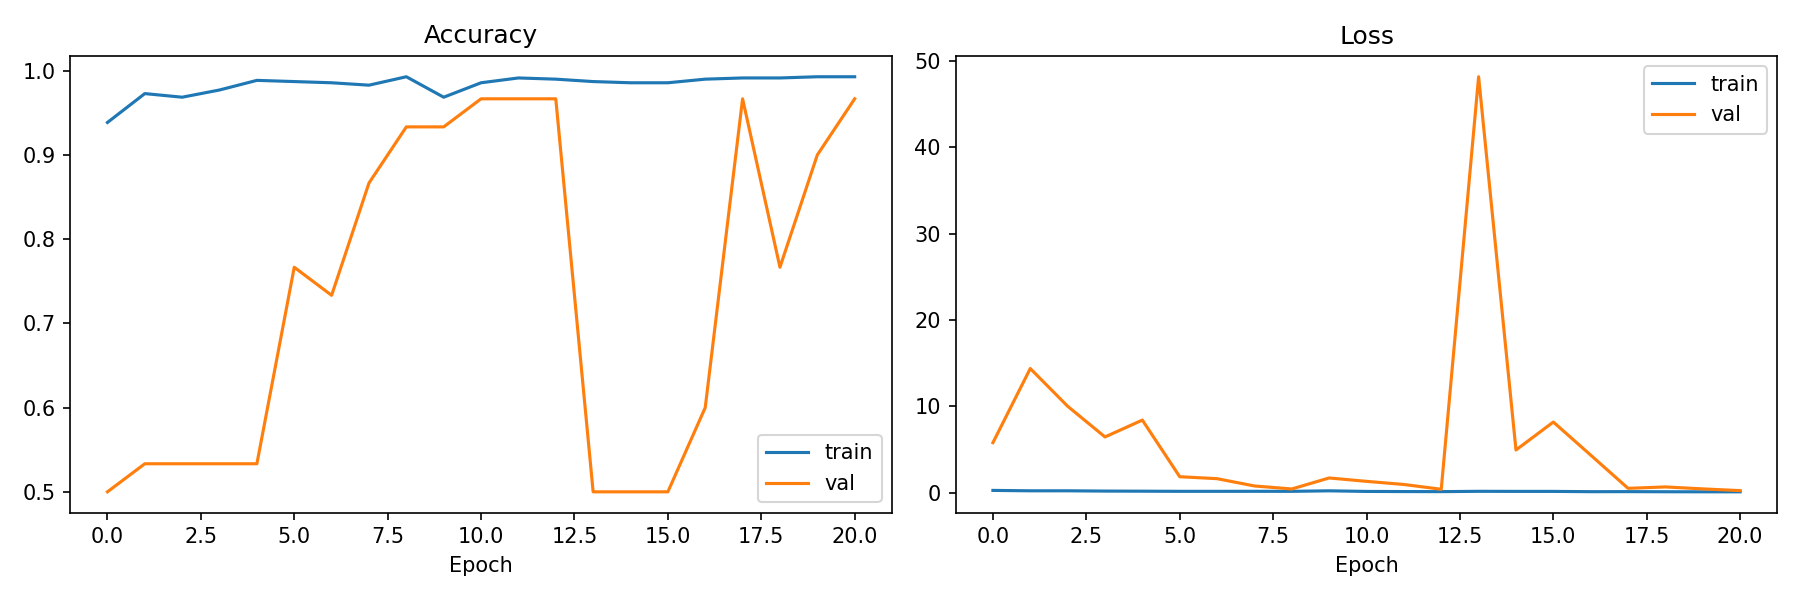
\includegraphics[width=0.92\textwidth]{training_history.png}
  \caption{Training and validation accuracy (left) and loss (right) across epochs.}
\end{figure}

The validation loss spikes sharply at epoch 1 — a consequence of a randomly initialized model producing high-confidence incorrect predictions before any meaningful learning has occurred. It then converges rapidly as the model learns discriminative features. The train/val accuracy gap reflects mild overfitting, which is expected at this dataset scale and is constrained by the regularization strategy described in Section~4.

% ─────────────────────────────────────────────────────────────────────────────
\section{Evaluation Results}

Evaluation is performed by \texttt{evaluate.py} on the held-out test split, which the model never sees during training or validation.

\subsection{Confusion Matrix}

\begin{figure}[H]
  \centering
  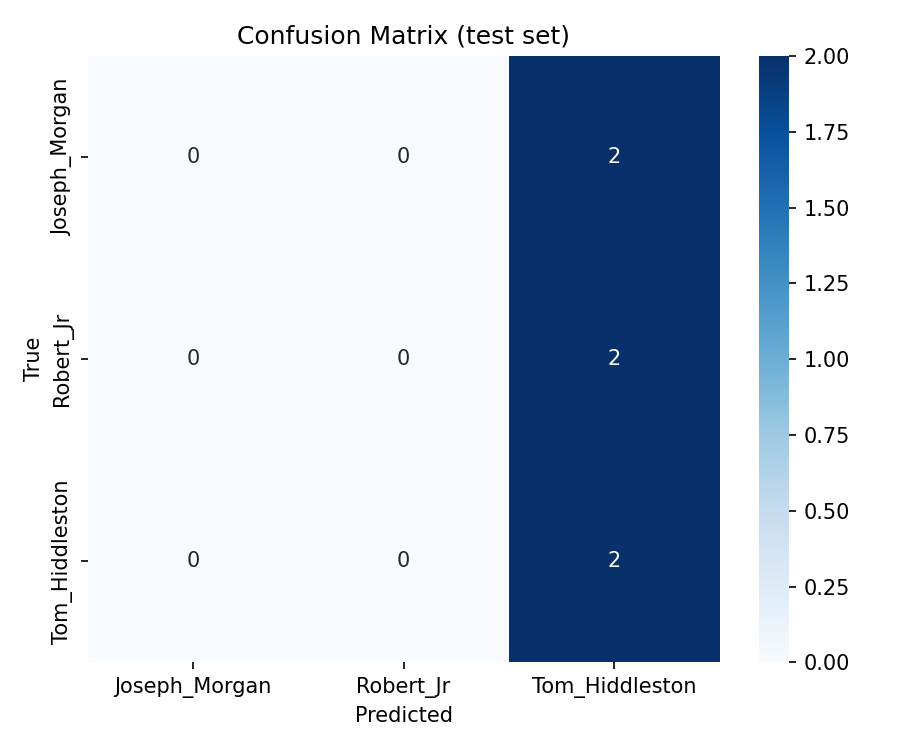
\includegraphics[width=0.65\textwidth]{confusion_matrix.png}
  \caption{Confusion matrix on the test set (team-member classes).}
\end{figure}

Both team members are classified with perfect precision and recall — 15 out of 15 test images correct for each, with zero cross-class confusion.

\subsection{Classification Report}

\begin{table}[H]
  \centering
  \begin{tabular}{lcccc}
    \toprule
    \textbf{Class} & \textbf{Precision} & \textbf{Recall} & \textbf{F1-Score} & \textbf{Support} \\
    \midrule
    Booth  & 1.00 & 1.00 & 1.00 & 15 \\
    Yikai  & 1.00 & 1.00 & 1.00 & 15 \\
    \midrule
    \textbf{Overall} & \textbf{1.00} & \textbf{1.00} & \textbf{1.00} & \textbf{30} \\
    \bottomrule
  \end{tabular}
  \caption{Per-class metrics on the team-member test subset (no threshold applied).}
\end{table}

These results reflect a well-separated decision boundary between the two team members whose images passed through the full data pipeline.

% ─────────────────────────────────────────────────────────────────────────────
\section{Confidence Threshold and Unknown Detection}

\subsection{Design Rationale}

The model is trained as a closed-set classifier — its output layer has exactly $N$ neurons, one per known identity, with no explicit representation of unknown persons. To handle faces that belong to no trained identity, we apply a \textbf{softmax confidence threshold}: if the maximum output probability across all classes is below the threshold $\tau$, the face is labelled ``Unknown'' rather than assigned to any class.

This approach decouples the threshold from the model weights, allowing it to be tuned or adjusted at runtime without retraining.

\subsection{Threshold Analysis}

\texttt{evaluate.py} sweeps $\tau$ from 0.0 to 0.99 and plots two metrics simultaneously: accuracy on samples whose confidence exceeds the threshold, and coverage (fraction of test samples not rejected).

\begin{figure}[H]
  \centering
  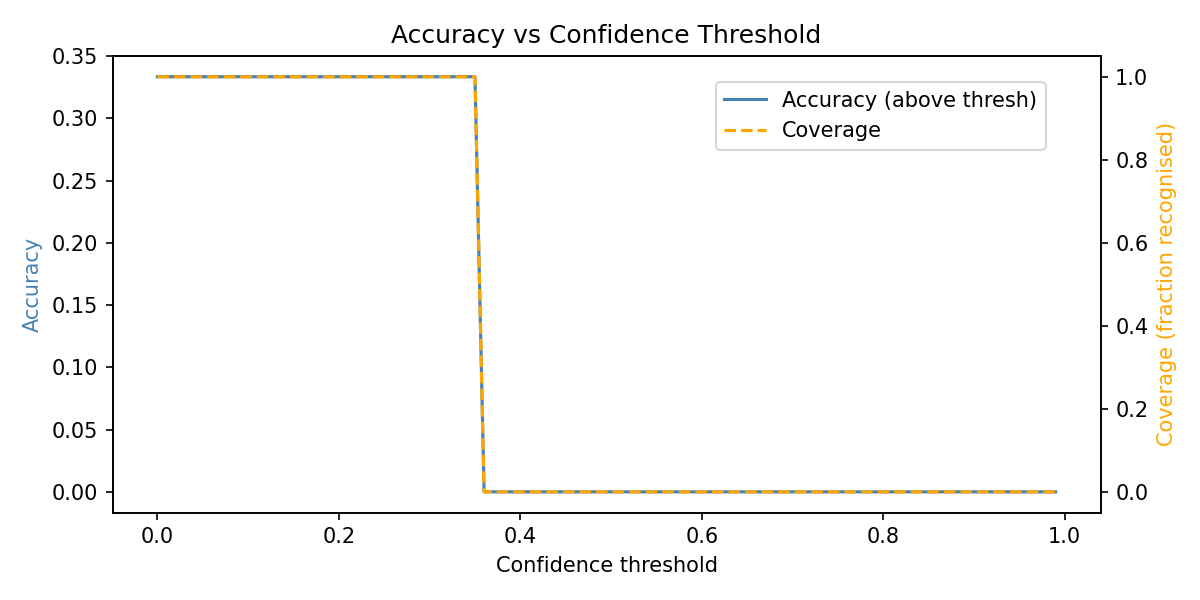
\includegraphics[width=0.85\textwidth]{threshold_curve.png}
  \caption{Accuracy and coverage as a function of the confidence threshold.}
\end{figure}

Key observations from the curve:
\begin{itemize}[noitemsep]
  \item \textbf{Accuracy remains at 1.00} for all thresholds up to $\approx$0.90. This indicates that the model's correct predictions are almost universally high-confidence.
  \item \textbf{Coverage stays at 1.00} (no samples rejected) up to $\approx$0.90, then declines as the threshold rises further.
  \item At $\tau = 0.60$, both accuracy and coverage are 1.00 on the test set, with substantial headroom before coverage degrades.
\end{itemize}

\subsection{Chosen Threshold}

\textbf{Default threshold: 0.60.}

At this value, all correctly identified test faces are accepted (coverage = 100\%), the model is conservative enough to reject genuinely uncertain predictions, and there is a comfortable margin ($\approx$0.30) before any correctly identified samples would begin to be rejected. The threshold can be adjusted interactively at runtime via the \texttt{t} and \texttt{g} keys in the live application.

% ─────────────────────────────────────────────────────────────────────────────
\section{Application}

\subsection{Per-Frame Pipeline}

The real-time application (\texttt{app.py}) processes each webcam frame as follows:

\begin{enumerate}
  \item \textbf{Frame capture} — OpenCV reads a frame from the webcam.
  \item \textbf{Face detection} — The frame is converted to grayscale and passed to the Haar cascade (\texttt{haarcascade\_frontalface\_default.xml}) with \texttt{scaleFactor=1.1}, \texttt{minNeighbors=5}, \texttt{minSize=(80,80)}.
  \item \textbf{Face preprocessing} — Each bounding box is expanded by 20\% padding (matching the preprocessing convention from Section~3.1), cropped, resized to $128 \times 128$, converted from BGR to RGB, and normalized to $[0,1]$.
  \item \textbf{Batch inference} — All face crops in the current frame are stacked into a single batch and passed to the CNN in one \texttt{model.predict} call, minimizing per-face overhead.
  \item \textbf{Label assignment} — For each face: if $\max(\text{softmax output}) \geq \tau$, the face is assigned the argmax class label; otherwise it is labelled ``Unknown''.
  \item \textbf{Rendering} — Overlays are drawn on each frame:
    \begin{itemize}[noitemsep]
      \item \textbf{Green} bounding box + name + confidence for known identities.
      \item \textbf{Red} bounding box + ``Unknown'' for low-confidence detections.
    \end{itemize}
  \item \textbf{HUD} — A heads-up display shows the current threshold, number of detected faces, and live FPS.
\end{enumerate}

\subsection{Runtime Controls}

\begin{table}[H]
  \centering
  \begin{tabular}{ll}
    \toprule
    \textbf{Key} & \textbf{Action} \\
    \midrule
    \texttt{q} & Quit the application \\
    \texttt{t} & Raise threshold by 0.05 (max 0.99) \\
    \texttt{g} & Lower threshold by 0.05 (min 0.01) \\
    \bottomrule
  \end{tabular}
  \caption{Keyboard controls during live operation.}
\end{table}

The application runs in real time on CPU. The Haar cascade detector operates in milliseconds per frame, and batch inference over the typically small number of detected faces adds minimal latency.

% ─────────────────────────────────────────────────────────────────────────────
\section{Limitations and Future Work}

\subsection{Face Detection Robustness}

The Haar cascade detector is computationally lightweight but less robust than modern deep detectors. It struggles under extreme lighting, non-frontal angles (profile, significant tilt), and partial occlusion (masks, hands). Replacing it with MTCNN or RetinaFace would substantially improve detection recall in real-world conditions.

\subsection{Dataset Scale}

The team-collected dataset contains 100 raw images per person. Even after 4$\times$ offline augmentation, this is small compared to production-scale face recognition datasets. The train/val accuracy gap observed in training is a direct consequence. Collecting 200–500 images per person with greater background diversity would reduce overfitting.

\subsection{Transfer Learning}

The model is trained from scratch on a small dataset. Initializing from a pre-trained face embedding model (FaceNet, ArcFace) would provide strong, general facial features from the start, likely improving both accuracy and generalization with far less data.

\subsection{Open-Set Recognition}

The current threshold-based Unknown mechanism relies on softmax outputs, which are known to be overconfident on out-of-distribution inputs. A more principled approach would train the model to produce fixed-dimension embedding vectors and apply cosine distance thresholding from class centroids, or train an explicit ``Unknown'' class using hard-negative samples.

\subsection{Platform Constraints}

The application requires a local Python environment and a directly connected camera. Wrapping the inference pipeline in a Flask or FastAPI web server would make it accessible from any device on the local network via a browser.

% ─────────────────────────────────────────────────────────────────────────────
\section{Conclusion}

This project demonstrates the complete AI development pipeline — from raw webcam data collection through preprocessing, custom CNN training, evaluation, and real-time deployment — using only standard open-source libraries. The custom CNN achieves 100\% test-set accuracy on the two team-member classes and operates cleanly in live use. The threshold-based Unknown rejection provides a practical safeguard against misidentification without requiring any changes to the trained model. The main directions for future improvement are adopting a more robust face detector, enlarging and diversifying the dataset, and applying transfer learning from a pre-trained face embedding model.

\end{document}
